%%% template.tex
%%%
%%% This LaTeX source document can be used as the basis for your technical
%%% paper or abstract. Intentionally stripped of annotation, the parameters
%%% and commands should be adjusted for your particular paper - title, 
%%% author, article DOI, etc.
%%% The accompanying ``template.annotated.tex'' provides copious annotation
%%% for the commands and parameters found in the source document. (The code
%%% is identical in ``template.tex'' and ``template.annotated.tex.'')

\documentclass[conference]{acmsiggraph}

\usepackage{amsfonts}
\usepackage{amssymb}
\usepackage{amsmath}
\usepackage[]{graphicx}
\usepackage{hyperref}
\usepackage{subcaption}
\usepackage{float}

\TOGonlineid{45678}
\TOGvolume{0}
\TOGnumber{0}
\TOGarticleDOI{1111111.2222222}
\TOGprojectURL{}
\TOGvideoURL{}
\TOGdataURL{}
\TOGcodeURL{}

\title{Lighting estimation for different time periods using light probes}

\author{
  Caio F. Valente\\
  \texttt{caiov@ime.usp.br}
  \and
  Thiago G. Nunes\\
  \texttt{nunes@ime.usp.br}
}
\pdfauthor{Caio F. Valente}
\pdfauthor{Thiago G. Nunes}

\keywords{image based lighting, global illumination}

\begin{document}

%% \teaser{
%%   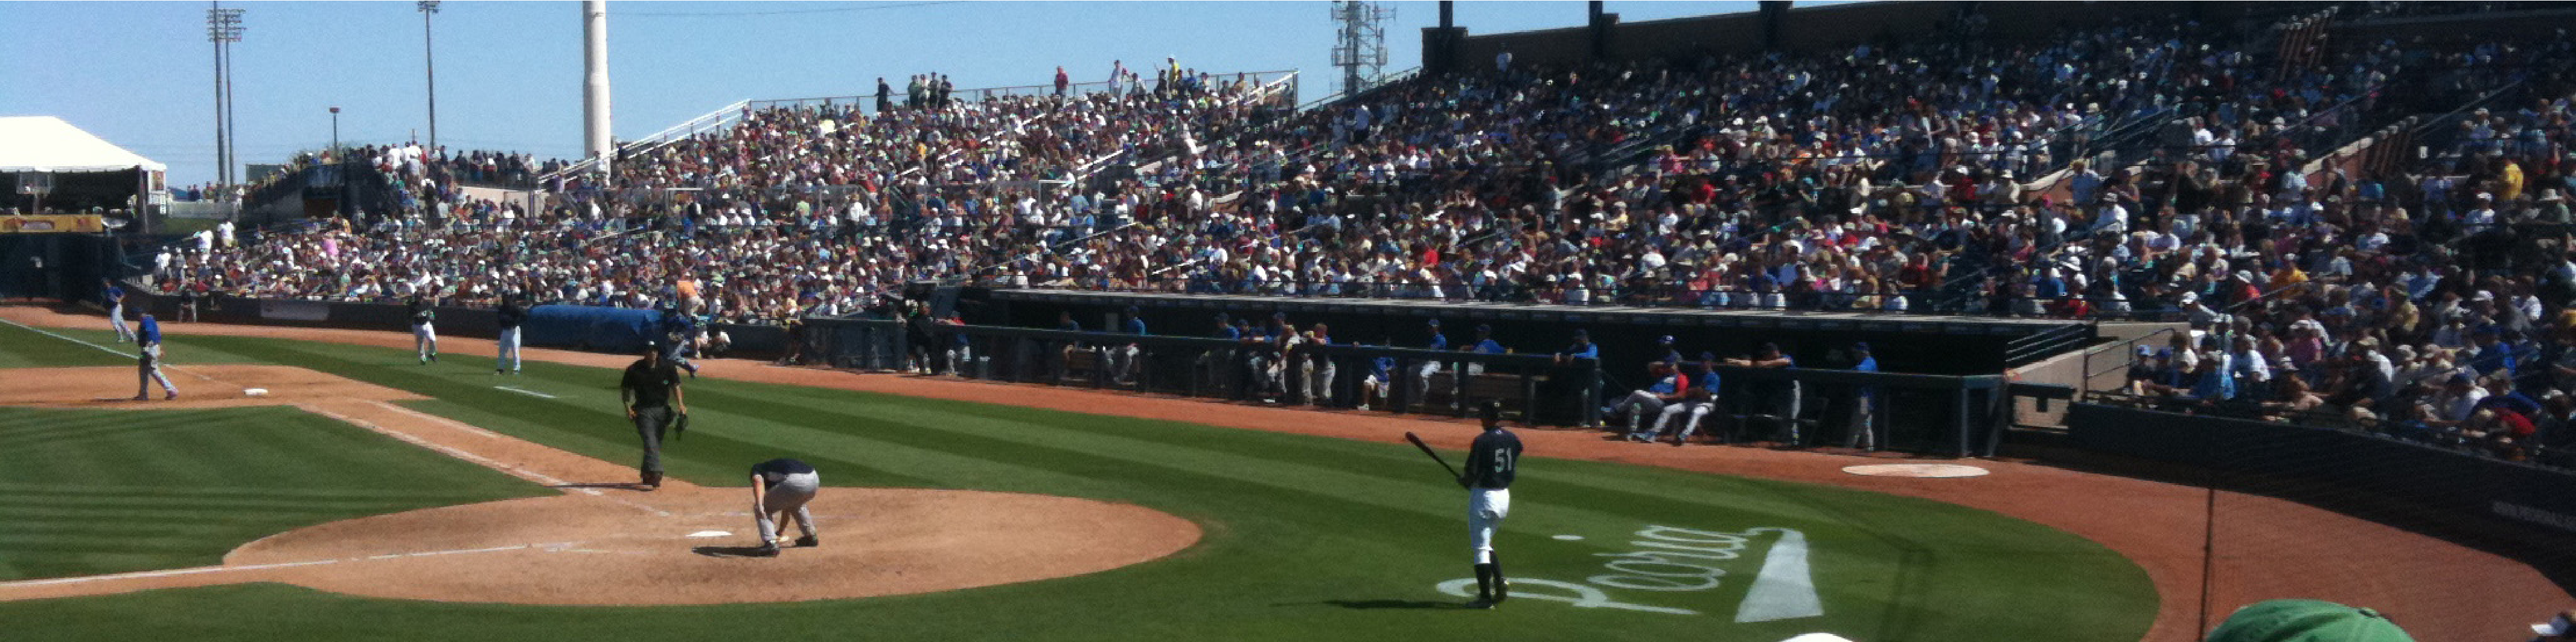
\includegraphics[height=1.5in]{images/sampleteaser}
%%   \caption{Spring Training 2009, Peoria, AZ.}
%% }

\maketitle

\begin{abstract}
	In this paper, we present a way to approximate real lighting for different time periods by using image based lighting with sparsely obtained light probes. In order to maintain 
	lighting consistency we use of interpolation, we have tested and compared a few interpolation methods.
\end{abstract}

\begin{CRcatlist}
  \CRcat{I.3.3}{Computer Graphics}{Three-Dimensional Graphics and Realism}{image based lighting}
  \CRcat{I.3.7}{Computer Graphics}{Three-Dimensional Graphics and Realism}{global illumination};
\end{CRcatlist}

\keywordlist

%% Use this only if you're preparing a technical paper to be published in the 
%% ACM 'Transactions on Graphics' journal.

\TOGlinkslist

%% Required for all content. 

\copyrightspace

\section{Introduction}

Computer graphics is present in a wide variety of areas ranging from entertainment to medicine or military applications, and one of its biggest challenges is generating realistic and 
convincing synthetic scenes. Realistic scene synthesis is dependent on a few factors, like geometry, materials and lighting. One of the most complex elements to reproduce are those 
related to lighting.

We would like to render scenes in different periods of the day with realistic and convincing lighting. Realistic lighting can be achieved by means of a technique called IBL – Image 
Based Lighting. 

Image Based Lighting consists in obtaining light probes, which are omnidirectional High Dynamic Range images, and using them as environment maps during the rendering phase.

However, this technique is limited in the sense that we must obtain a new light probe for every instant we would like to render. This limitation makes the use of image-based lighting 
inviable depending on the time range of the scenes to be rendered due to enormous amount of work involved in obtaining the light probes.

Our main goal is to alleviate the restriction that a light probe must be obtained for every moment to be rendered. In order to do that we propose the use of interpolation to estimate 
the light probes for the instants that data is not available.

We propose two comparisons to validate our approximation:
\begin{itemize}
	\item Comparing light probes obtained through interpolation and light probes obtained through the usual way, which is done by combining different exposure time images.
	\item Comparing the rendering a simple object using the interpolated light probe as a light source and the same object in the real scene. The object is a white cube \ref{fig:whitecube}.
\end{itemize}

\begin{figure}[!ht]
	\caption{Image obtained by using a fisheye lens.}
	\centering
	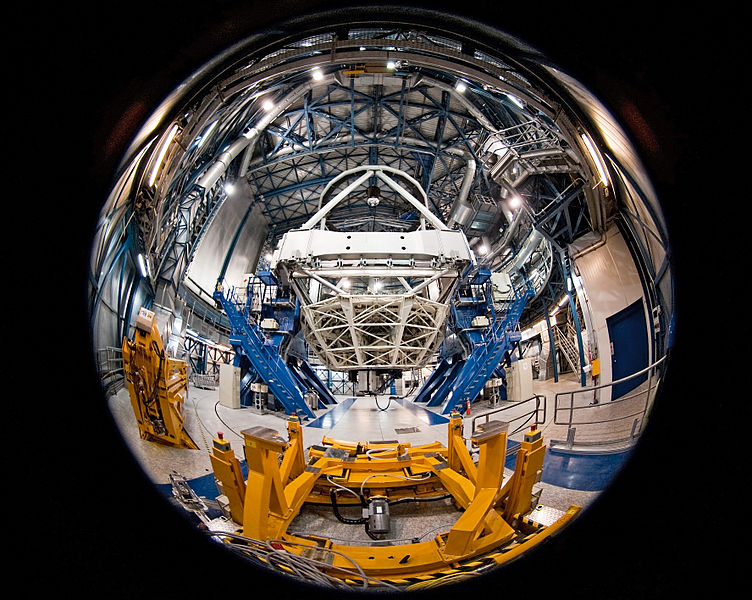
\includegraphics[width=7cm]{images/fisheye.jpg}
	\label{fig:whitecube}
\end{figure}

\section{Definitions}

\subsection{Environment Map}

	Environment mapping \cite{hughes2013} consists in exchanging the illumination model for a texture lookup model which contains the lighting information.

\subsection{High Dynamic Range}

	High Dynamic Range (HDR) is an image format capable of representing a scene’s great variation in luminosity. It is usually stored using floating points with 32 bits per channel. 
	HDR images can be obtained by using special cameras like the Spheron \cite{spheron}, or combining images with different exposure times using software like Photoshop or HDR Shop. 
	A scene’s radiance can be recovered from a scene’s HDR image \cite{debevec1997}.

\subsection{Image Based Lighting}

	Image Based Lighting (IBL) \cite{debevec2002} consists in capturing a scene illumination information through an omnidirectional HDR image. To capture omnidirectional images either 
	a reflective sphere (Figure \ref{fig:lightprobe}\cite{linda2007}) or fisheye lenses (Figure \ref{fig:fisheye}\cite{salgado2010}) can be used. The resulting image, called light probe, is then used as an environment 
	map in the rendering phase. Note that a new light probe must be acquired for different locations or periods, otherwise the lighting consistency might not be maintained.

	\begin{figure}[!ht]
		\caption{Image obtained by using a fisheye lens.}
		\centering
		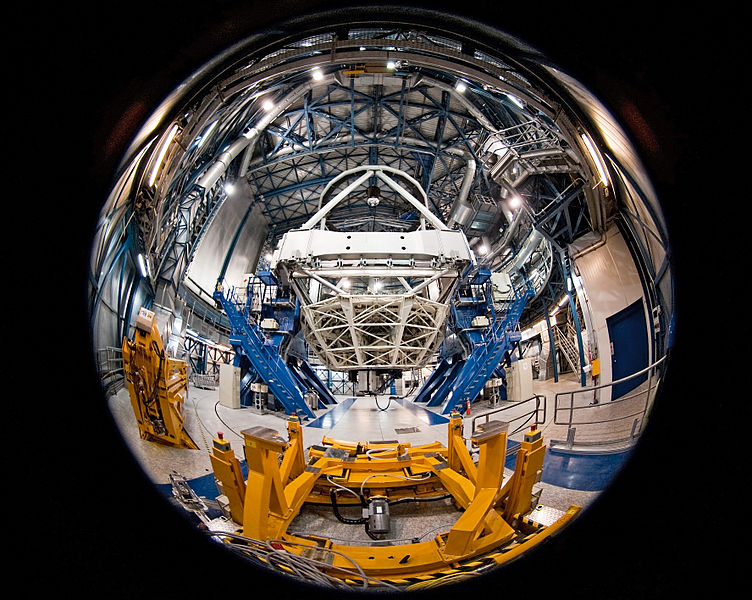
\includegraphics[width=7cm]{images/fisheye.jpg}
		\label{fig:fisheye}
	\end{figure}

	\begin{figure}[!ht]
		\caption{Reflective sphere that could be used as a light probe.}
		\centering
		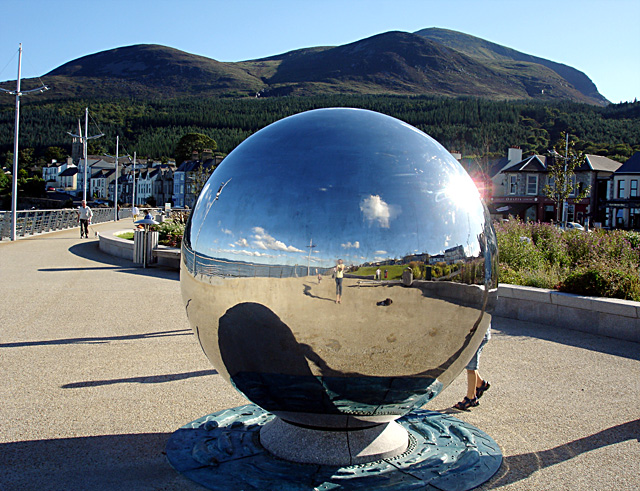
\includegraphics[width=7cm]{images/lightprobe.jpg}
		\label{fig:lightprobe}
	\end{figure}

\subsection{Interpolations}
	We have used five types of  interpolations to generate new light probes from our data. The light probes were interpolatate using pixel intensities over time.
\subsubsection{Linear Interpolation}
	The first interpolation is the classic linear interpolation. It's formula is as below: 
\begin{align}
	y' = y_0 + (y_1-y_0)*\frac{x-x_0}{x_1-x_0}
\end{align}
Where $y$ represents the intensities of each pixel while $x$ represents the time associated with the light probe's acquisition.

\subsubsection{Gauss Foward Central Difference Formula}
	The second interpolation method is the Gauss Foward Central Difference Formula. Given a set of $n$ light probes, acquired at a regular time interval $h$, 
$(\dots,y_{i-2},y_{i-1},y_i,y_{i+1},y_{i+2},\dots)$ with acquisition times $(\dots,x_{i-2},x_{i-1},x_i,x_{i+1},x_{i+2},\dots)$, we can interpolate a new
light probe using the following formula:
\begin{align}
\begin{split}
	p' &= p_i + T \delta_{1/2} + G_2 \delta_0^2 + G_3 \delta_{1/2}^3 + \dots\\
	T &= (t-t0)/h \\
	G_{2n} &= \binom{T+n-1}{2n} \\
	G_{2n+1} &= \binom{T+n}{2n+1}
\end{split}
\end{align}
	The Foward interpolation uses an iterative method that adds the $n$-esieme central difference\cite{abramowitz1972handbook} using the piramidal construction showed by Figure \ref{fig:fowardcentral}.

\begin{figure}[!ht]
	\caption{Reflective sphere that could be used as a light probe.}
	\centering
	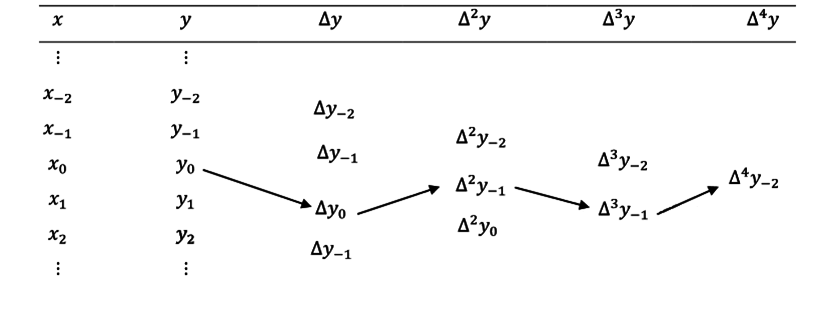
\includegraphics[width=10cm]{images/forward.png}
	\label{fig:fowardcentral}
\end{figure}

\subsubsection{Gauss Backward Central Difference Formula}
	The Gauss Backward Central Difference Formula differ from the Foward because it's uses 

\section{Experiment}

\section{Results}

\section{Conclusion}

\section*{Acknowledgements}

\bibliographystyle{acmsiggraph}
\bibliography{template}
\end{document}
